\chapter{Implementazione e realizzazione del sistema}
\label{capitolo5}
\thispagestyle{empty}



\noindent All'interno di questo capitolo verranno illustrate tutte le tecniche implementative per realizzare quanto è stato enunciato nel capitolo precedente. Nel dettaglio verranno spigate, argomentate le implementazioni effettuate su tutte le fasi della tesi, i riferimenti teorici che hanno permesso la realizzazione di questa tesi. Di seguito una breve descrizione grafica del flusso con le operazioni effettuate durante la redazione del lavoro di tesi.(vedi fig:\ref{Flusso})
\begin{figure}[h!]
    \begin{center}
      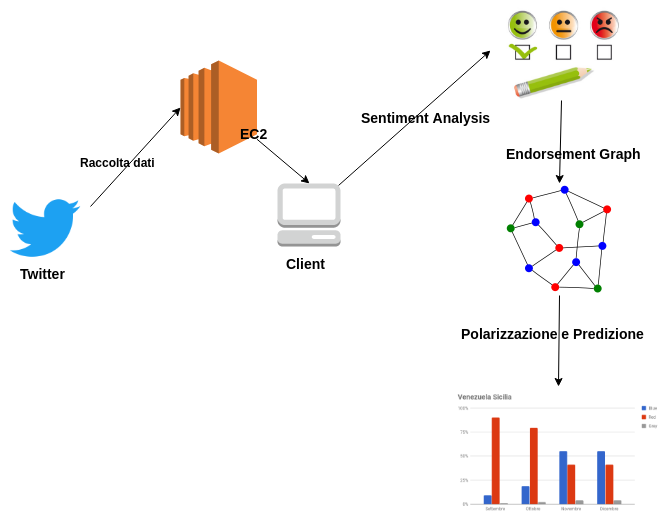
\includegraphics[scale= 0.5]{Flusso.png}
	%
\psfig{file=./pictures/logo}
	\caption{Flusso}
	\label{Flusso}
    \end{center}
  \end{figure}

\section{Raccolta dati}
\label{raccolta}
La raccolta dati è la fase iniziale della tesi di laurea. Come precedentemente argomentato il social network di riferimento utilizzato è \textit{Twitter}.Prima di spiegare quanto fatto occorre citare le funzionalità della \textit{Twitter Api}. Successivamente verranno illustrate le tecniche adottate per la raccolta dei \textit{Tweet} del passato.
\subsection{Twitter Api}
Sono delle api messe a disposizione dal social network Twitter, per poterle utilizzare occorre necessariamente effettuare l'iscrizione al reparto sviluppatori di Twitter, mettendo a disposizione il proprio account personale, quindi come prima cosa occorre predisporre di un proprio account. La raccolta dei dati può essere effettuata soltanto dopo aver abilitato l'account. Per raccogliere i dati pubblicati dagli utenti all'interno della rete occorre creare una \textit{Twitter Apps}, la quale rilascerà delle credenziali che dovranno essere utilizzate per poter effettuare le richieste attraverso le Twitter Api al server. Viene inizializzato un processo di streaming tra il client ed il server che consenta la ricezione dei dati, diamo una definizione delle credenziali, che sono divise in:
% Tale operazione viene eseguita attraverso un processo di streaming, questa operazione occorre creare una \textit{Twitter Apps} il quale rilascerà una volta creata una serie di codici che dovranno essere utilizzati per poter effettuare le richieste con le Twitter Api al server.
%Le credenziali sono divise in:
\begin{itemize}
\item \textit{Token}: identificano il token di accesso ai servizi messi a disposizione da Twitter, a sua volta è composto da:
\begin{itemize}
\item \textit{Access token}
\item \textit{Access secret}
\end{itemize}
\item \textit{Consumer}: è un codice di accesso ai servizi di consumo, ovvero consente lo streaming dei dati dal server, si suddivide in due chiavi:
\begin{itemize}
\item \textit{Consumer key}
\item \textit{Consumer secret}
\end{itemize}
\end{itemize}
Queste chiavi di accesso possono essere generate più e più volte, una volta creata un'applicazione per lo sviluppo di Twitter.
Le Api sono disponibili in diversi linguaggi di programmazione tra cui il \textit{Python}, utilizzato per lo sviluppo della tesi.
Per richiamare tutte le api attraverso il codice è necessario sempre autenticarsi, caricando le credenziali di accesso  fornite attraverso i permessi da sviluppatore precedentemente illustrate.
Lo streaming per la raccolta dei dati è soggetto a stringenti regole per evitare un uso improprio delle informazioni diffuse dagli utenti all'interno della rete. Infatti c'è un numero massimo di richieste che un utente, con le credenziali da sviluppatore, può effettuare, cioè 100 ogni 15 minuti. Allo scadere di tale tempo potrà ricominciare, altrimenti nel caso in cui un utente non tenesse conto di questa limitazione ed effettuasse una nuova richiesta durante il tempo di pausa le sue credenziali verrebbero bloccate per circa un'ora non potendo più interagire con le api di Twitter.
La risposta da parte del server sarà un file \textit{JSON} contenente tutti i metadati dell'utente in questione, come il testo del Tweet, il suo id, lo username dell'utente che ha effettuato il tweet, i mentions gli hashtag ed il numero di retweet con la lista degli utenti che hanno retwettato la notizia in questione.

\subsection{Get Old Tweet}
Questa sezione illustrerà in che modo sono stati raccolti tutti i tweet del passato. Avendo spiegato nella sezione precedente le problematiche relative al numero di richieste da effettuare nell'arco temporale, è stata seguito un approccio differente che consentiva di limitare il numero di richieste alla volta.
L'approccio in questione consiste nell'effettuare una \textit{GET} sulla pagina di ricerca di Twitter, specificando l'argomento ricercato, ed il periodo di validità della ricerca.
Twitter suddivide gli account abilitati allo sviluppo in 3 categorie:
\begin{itemize}
\item \textit{Standard}: account gratuito soggetto a limitazione temporali e sui contenuti, non è possibile ricercare tweet precedenti a 7 giorni. I dati richiesti non sono completi.
\item \textit{Premium}: account a pagamento con sole limitazioni temporali, non è possibile ricercare tweet precedenti a 30 giorni. Non ha nessun problema di completezza sui contenuti.
\item \textit{Enterprise}: account a pagamento senza alcuna limitazione temporale e sui contenuti.
\end{itemize}
Avendo utilizzato un account \textit{Standard} sono stati ricercati dei metodi per poter risolvere le problematiche precedentemente descritte, cercando di ottenere più informazioni possibili.
%Un altro problema che ha spinto all'utilizzo di questo metodo riguarda la politica di Twitter nel far collezionare, agli utenti non premium con i permessi di sviluppo, soltanto i dati con data di riferimento di 7 giorni precedenti alla data di ricerca selezionata. Per di più come indicato all'interno della documentazione i dati raccolti mediante le Twitter Api non saranno tutti quelli pubblicati nel periodo selezionato.

Tutte queste problematiche sono state risolte la libreria \textit{Get Old Tweet}, il quale crea un indirizzo http con i parametri di ricerca richiesti, nel nostro caso:
\begin{itemize}
\item \textit{La query}: la parola chiave, l'hashtag da ricercare all'interno dei Tweet.
\item \textit{Data inizio}: la data in cui inizio a raccogliere i dati.
\item \textit{Data Fine}: la data in termino la ricerca e la raccolta dei dati.
\end{itemize}
Una volta definiti questi parametri all'interno della \textit{url}, viene restituita la pagina html contenente tutti i  tweet presenti nel periodo indicato. Il risultato verrà convertito in un formato \textit{json}, per estrarre le informazioni basterà parsare la pagina ottenendo i seguenti dati:
\begin{itemize}
\item Lo \textit{username} della persona che ha postato il tweet.
\item Il numero di \textit{retweet} al tweet. 
\item Il \textit{testo} del tweet pubblicato.
\item La lista  degli \textit{hashtag} pubblicati dall'utente all'interno del tweet
\item La lista dei \textit{mentions} pubblicati dall'utente all'interno del tweet.
\item La \textit{data} di pubblicazione del tweet.
\end{itemize}
Per far comprendere meglio queste informazioni nell'immagine sovrastante viene presentato un tweet di esempio con le informazioni precedentemente elencate, per far comprendere al meglio gli elementi in questione.
\begin{figure}[h]
    \begin{center}
      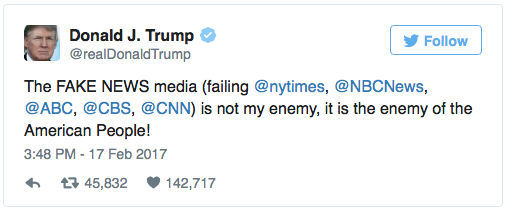
\includegraphics[scale= 0.8]{trump.png}
	%
\psfig{file=./pictures/logo}
	\caption{esempio Tweet}
    \end{center}
  \end{figure}
  
Tutti questi dati sono stati successivamente elaborati ed analizzati. Particolare attenzione è stata posta a due di essi ovvero: il testo ed il numero di retweet. 
Il primo per effettuare la sentiment analysis e poter definire una prima partizione dei dati, che andranno a generare il grafo.
Il secondo perché costituisce la base per i nuovi nodi del grafo e quindi la diffusione del tweet con altri utenti. 
Per identificare la lista degli utenti che hanno effettuato il retweet sul tweet in questione è stato necessario usare una libreria chiamata \textbf{Tweepy}.
Questa libreria sfrutta le \textit{Twitter Api}, effettuando delle chiamate rest sul server di Twitter per ricevere le informazioni richieste. Nel nostro caso è stato utilizzato il metodo \textit{retweet} che ricevendo come argomento l'id relativo al tweet pubblicato permette di ricevere la lista degli username che hanno pubblicato quell'argomento all'interno della propria rete. Il problemi presentati in precedente nell'utilizzare queste chiamate al server sono sempre validi, infatti se vengono superate le 100 richieste viene lanciata un'eccezione: \textit{Tweepy Error} che consente di mettere in pausa l'applicazione attraverso una sleep per 15 minuti. Una volta terminato il tempo di attesa la richiesta viene ripresa dal punto richiesto, continuando a collezionare gli username richiesti.
Tutti i dati raccolti durante le operazioni di streaming sono stati salvati all'interno di un file binario per poter ottimizzare lo spazio fisico.

\subparagraph{EC2}
La raccolta dati utilizzando le implementazioni precedentemente citate, è stata eseguita all'interno di una istanza \textbf{EC2}. 
Il motivo di tale scelta è dettata dai tempi di attesa via via sempre più lunghi per la raccolta degli username degli utenti che hanno retweettato i tweet raccolti, per via delle politiche stringenti dettate da \textbf{Twitter}.  Utilizzando un'istanza a pagamento, si è dovuto ottimizzare il salvataggio fisico dei dati, perché oltre ad essere un servizio a consumo di risorse di calcolo, vengono pagate anche i dati salvati all'interno dello storage fisico della macchina. Attraverso la libreria \textit{pickle}\footnote{libreria per il salvataggio dei dati fornita da \textit{Python}} si è potuto risolvere questo problema, in quanto ottimizza il salvataggio dei dati attraverso una conversione in binario degli stessi.


\section{Sentiment Analysis}
\label{Sentiment}
La sentiment analysis è l'approccio utilizzato per la divisione dei diversi tweet, raccolti per un determinato topic, in un determinato periodo, analizzando il "sentimento" espresso nel contenuto del testo pubblicato dagli utenti.
Questa fase viene effettuata al momento della raccolta dei dati, cioè una volta collezionati l'insieme dei dati vengono sottoposti alla funzione implementata e salvati in due categorie distinte mediante la libreria \textit{pickle}, precedentemente illustrata.

L'implementazione di questo metodo è stata effettuata seguendo un approccio basato su \textit{metodi statistici}: questi metodi si basano su elementi di apprendimento automatico. Per misurare l'opinione nel contesto e trovare la caratteristica che è stata giudicata, sono usate le relazioni grammaticali delle parole utilizzate. Le relazioni di dipendenza grammaticale sono ottenute attraverso la scansione approfondita del testo. Il processo di apprendimento da parte della macchina (anche detto machine learning) non è immediato, devono infatti essere costruiti dei modelli che associano a diverse tipologie di commenti una polarità e se necessario ai fini dell'analisi anche un topic.

Si può riassumere quanto sviluppato attraverso la seguente immagine:
\begin{figure}[!h]
    \begin{center}
      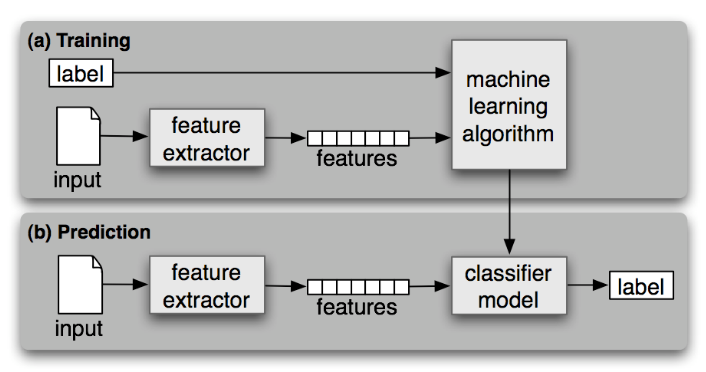
\includegraphics[scale= 0.55]{sentiment.png}
	%
\psfig{file=./pictures/logo}
	\caption{schema Sentiment Analysis}
    \end{center}
  \end{figure}
 
 Da quanto si evince dall'immagine mostrata risulta evidente quanto un meccanismo di \textit{machine learning} necessiti di un classificatore molto preciso. La precisione può essere ottenuta attraverso dei \textit{training set}, ovvero dei file che istruiscano la macchina permettendo una classificazione ottimale dei dati.
Ci sono diversi classificatori, quello utilizzato per l'implementazione della Sentiment Analysis è descritto di seguito.
\begin{itemize}
\item \textbf{classificatore Naive Bayes}:
Un classificatore bayesiano è un classificatore basato sull'applicazione del teorema di Bayes.
Richiede la conoscenza delle probabilità a priori e condizionali relative al problema, quantità che in generale non sono note ma sono tipicamente stimabili. Se è possibile ottenere delle stime affidabili delle probabilità coinvolte nel teorema, il classificatore bayesiano risulta generalmente affidabile e potenzialmente compatto. Per costruzione, il classificatore bayesiano minimizza il rischio di classificazione.

Nel gergo della classificazione di testi o \textit{Text Categorization}, con il termine classificatore bayesiano ci si riferisce convenzionalmente al classificatore Naive Bayes, ossia un classificatore bayesiano semplificato con un modello di probabilità sottostante che assume l'indipendenza delle \textit{feature}, ovvero che la presenza o l'assenza di una particolare \textit{feature} in un documento testuale non è correlata alle altre.

L'esperienza dimostra che il metodo funziona in molti problemi pratici, come per esempio il filtraggio antispam adattivo. Un vantaggio del classificatore Naive Bayes è che richiede solo un training set di esigue dimensioni per stimare i parametri necessari per la classificazione.

\end{itemize}

Tornando allo sviluppo, la prima operazione fatta è stata quella di raccogliere dati per classificare i tweet secondo un determinato topic. Questa operazione è stata effettuata manualmente anche per permettere alla macchina di poter riconoscere l'ironia, cosa che è possibile solo per la mente umana.Per questo motivo la precisione dei classificatori non sarà mai assoluto, conseguentemente le macchine necessitano dell'intervento dell'uomo per risolvere tali problematiche. Il training set in questione è stato redatto attraverso un file csv (vedi tabella: \ref{training}) costruito con due colonne:
\begin{itemize}
\item \textit{label}: ovvero l'identificatore che verrà utilizzato nell'analisi del classificatore per analizzare il contenuto di tweet ed associarlo ad un gruppo piuttosto che ad un altro.
\item \textit{Tweet}: il testo del tweet pubblicato, contenente anche caratteri speciali, elementi multimediali, link etc.
\end{itemize}
%Inserire una tabella con un esempio dei tre valori
\begin{table}[!htb]
\centering

\begin{tabular}{ |p{3cm}|p{7cm}| }
 \hline
 \multicolumn{2}{|c|}{\textbf{Training set}} \\
 \hline 
 \begin{center}
 \textbf{Label}
 \end{center} & \begin{center}
 \textbf{Tweet}
 \end{center}\\
 \hline
 5stelle   & Chi ama la sua terra non può che votare il \#M5S \#Regionali \#Sicilia pic.twitter.com/gv3CQWhCeI   \\
 ForzaItalia &   Con elezioni $ @matteosalvinimi$ e $@Musumeci\_Staff$ regionali 2017 in \#Sicilia !!\#elezioniregionali2017 \#andiamoagovernare \#forzalega  \\
Altri & Tutti gli schieramenti alle \#elezioniregionali in Sicilia.L'articolo di Pierangelo Bonanno \\
 \hline
\end{tabular}

\caption{Esempio di training set}
\label{training}
\end{table}
Una volta definito un training set occorre definire un \textit{vettore di Feature}:
\begin{itemize}
\item Rappresenta l'elemento cardine di un classificatore, maggiore è la sua efficienza e maggiore sarà la sua precisione. Il vettore di feature è utilizzato per costruire un modello che consenta, attraverso un training set, di poter fare una predizione sui dati che non ha mai analizzato prima.
Dovendo analizzare dei dati basati su Twitter si è deciso di adottare degli schemi basati sull'assenza o meno di alcune parole che appaiono nei tweet come feature. Attraverso il training set, composto da tweet suddivisi in 3 gruppi (positivi, negativi e neutrali)\footnote{Questa classificazione può essere modificata in base alle esigenze dell'utente, modificando i label nel file csv del \textit{training set}}, suddividiamo ciascun tweet in parole e aggiungeremo ogni parola la vettore di feature. Tale approccio viene definito \textit{unigrams}.Prima di andare ad inserire tali parole all'interno di questo vettore, andremo ad effettuare delle operazioni di filtraggio scartando quelle parole che non sono necessarie per comprendere il sentimento. 
Nel nostro caso le congiunzioni, articoli, preposizioni semplici ed articolate, ma anche altri caratteri perché generalmente i tweet contengono caratteri speciali come \textit{\# , @, link},  vengono inseriti all'interno della lista di parole di \textit{Stop}, cioè una lista popolata da tutte quelle parole che potrebbero far saturare il vettore di feature e che non esprimono un sentimento.
Il vettore di feature viene popolato a partire da tutte le parole che non sono presenti all'interno della lista di \textit{Stop} e che appartengono a tutti i tweet del training set.
\end{itemize}
 
In conclusione una volta definito il classificatore, il vettore di Feature ed il training set non resta che illustrare il calcolo della sentiment Analysis.
Per l'implementazione del classificatore \textit{Naive Bayes} si è utilizzata la libreria \textit{Python} \textbf{NLTK}\footnote{Natural Language Toolkit.}, la quale una volta istruito il classificatore attraverso il training set, precedentemente popolato in base alle proprie esigenze (come nell'esempio \ref{training}) utilizza il vettore di feature per ricercare la vicinanza del tweet al training set, restituendo il label corrispettivo (inserito dall'utente nella definizione del csv sopra citato). In questo modo sarà possibile sottoporre ogni testo dei diversi tweet raccolti al sistema il quale restituirà il responso in breve tempo. Per garantire una maggiore accuratezza nelle predizioni sarà necessario arricchire il training set con molteplici tweet. All'interno della sezione dedicata agli esperimenti verranno illustrati alcuni esempi dei label e dei tweet utilizzati per il calcolo dell'analisi illustrata all'interno di questa sezione. 

\section{Endorsement Graph}
In questa sezione verranno illustrate le tecniche e gli strumenti utilizzati per la realizzazione dell'\textit{endorsement graph}, cioè un grafo diretto che consenta la diffusione e la pubblicazione delle notizie.
Un grafo è un insieme di elementi chiamati nodi connessi tra di loro attraverso degli archi, essendo il nostro un grafo diretto significa che gli archi in questione hanno dei versi di orientamento da un nodo ad un altro.
Definiamo gli elementi costituenti:
\begin{itemize}
\item \textit{Nodo}: per ogni nodo è stato associato un utente che abbia pubblicato una notizia sul topic analizzato.
\item \textit{Arco}: per ogni arco è stata associata una relazione tra il tweet pubblicato da un nodo ed il retweet effettuato da un altro utente. Questi archi sono possono essere pesati, cioè avere una probabilità che una qualsiasi coppia di nodi sia adiacente. Nel nostro caso tale valore viene definito dalla \textit{probabilità di retweet}.
\end{itemize}

La creazione di questo grafo diretta dipende strettamente dai risultati ottenuti durante la raccolta dati. Nel dettaglio sono stati collezionati tutti i tweet che contenessero i 5 \textit{hashtag} più utilizzati per l'espressione del suddetto topic, una volta raccolta tutti i dati in questione questi sono stati fusi ed utilizzati per la definizione del grafo. I dati sono stati salvati in tre gruppi differenti grazie ai risultati ottenuti durante la \textit{Sentiment Analysis},questa classificazione risulta necessaria per la colorazione ed il calcolo della polarizzazione sul grafo. Tornando alla creazione è stata applicata una limitazione e cioè che i nodi isolati non venissero considerati all'interno del grafo. La motivazione che ha spinto nell'adottare tale politica è dettata dall'esigenza di ricercare quanto un idea espressa attraverso un tweet venga diffusa in un grafo e quanto questa sia polarizzata, quindi un nodo isolato che non viene ripubblicato dagli utenti risulta inutile ai fini dell'analisi in questione.
In precedenza nella definizione di Arco si è definita la probabilità di retweet:
\begin{quote}
Si definisce tale il rapporto che intercorre tra il numero dei retweet che l'utente ha effettuato su un nodo\footnote{Per nodo ci si riferisce ad un tweet pubblicato da un utente} con il numero di retweet totali effettuati dall'utente stesso.
\begin{equation}
 P(retweet)_{ij} = \dfrac{\#retweet_{ij}}{\#retweet_{j}} 
\end{equation}
 con i,j= nodi adiacenti appartenenti al grafo.
 \end{quote}
 Avendo raccolto dati da \textit{hashtag} differenti è possibile che alcuni utenti potessero retwettare lo stesso utente che avesse pubblicato nuovi tweet, per mantenere questa relazione si è incrementato il numero totale di retweet effettuati complessivamente così come il numero di volte che l'utente ha retwettato le opinioni di quello specifico utente. 

Prima di popolare il grafo sono state effettuate tutte le precedenti operazioni. La realizzazione del grafo è stata ultimata attraverso la libreria \textbf{Networkx}\footnote{NetworkX è una libreria Python per la creazione, manipolazione e studio delle strutture, dinamiche, e delle funzioni di una rete complessa.}, scritta in \textit{Python}.
Il grafo in questione può essere modificato graficamente, nel nostro caso per meglio far comprendere la polarizzazione si è deciso di adottare i colori: 	\textit{Rosso} e \textit{Blu}; per rappresentare le due partizioni raccolte attraverso la sentiment analysis, successivamente calcolarne la polarizzazione.(Vedi fig:\ref{endorsement})
%inserire un esempio grafico di un endorsement graph senza lab
\begin{figure}[!h]
    \begin{center}
      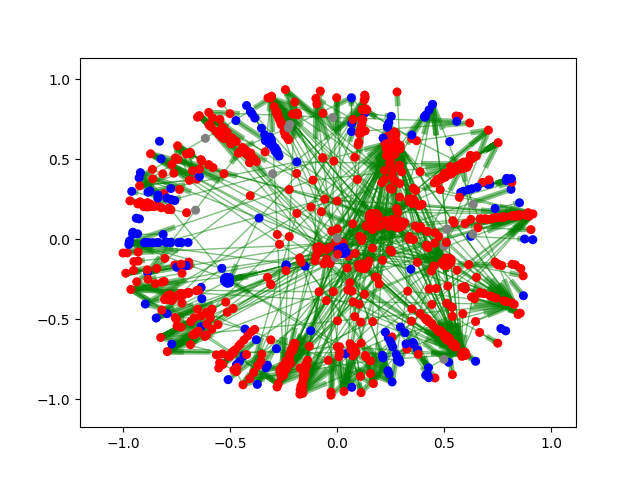
\includegraphics[scale= 0.8]{esempio.png}
		\caption{esempio di Endorsement Graph}
	\label{endorsement}
    \end{center}
  \end{figure}
\newpage
\section{Polarizzazione}
\label{Polarizzazione}
La polarizzazione viene definita come un processo sociale in cui un gruppo viene diviso: 
in due sottogruppi aventi un conflitto o una visione differente del problema in questione, e da alcuni individui che rimangono neutrali.
Dal punto di vista matematico la polarizzazione è una assegnazione di un valore compreso all'interno di un range:
\begin{equation}
[-1,1]
\end{equation}
I valori in questione identificano la vicinanza ad un gruppo piuttosto che ad un altro, in conclusione occorre assegnare alle due visioni contrastanti, che si vogliono analizzare, due valori di riferimento ovvero gli estremi.
Di seguito verranno illustrate le due implementazioni realizzate per il calcolo della polarizzazione all'interno di un endorsement graph.

\subsection{Polarizzazione basata sul grado}
All'interno di questa sezione verrà illustrata l'implementazione della polarizzazione attraverso l'algoritmo illustrato all'interno del paper: \textit{Measuring Political Polarization: Twitter shows the two sides of Venezuela}.

Come precedentemente spiegato all'interno di questa tesi, il primo passo consiste nell'individuare due tipi di nodi: 
\begin{itemize}
\item \textit{Elite}: sono i nodi che hanno pubblicato una notizia all'interno del grafo, sul topic selezionato.
\item \textit{Listener}: sono i nodi che seguono le informazioni pubblicate dai nodi \textit{Elite}.
\end{itemize}
Questa suddivisione è indipendente dai risultati ottenuti dalla sentiment analysis, cioè la prima partizione effettuata analizzando i contenuti, in questo modo si analizza la diffusione delle opinioni.
Illustriamo ora i passi algoritmici implementati per la realizzazione di questa polarizzazione:
\begin{enumerate}
\item Per prima cosa individuiamo tutti i nodi \textit{Elite} e quelli \textit{Listener}, per poter assegnare il primo valore della polarizzazione.
\begin{equation}
-1\leq X_{s}\leq1
\end{equation}
La formula precedentemente illustrata indica il range dei valori che la polarizzazione può assumere all'interno del grafo. 
\item Il passo successivo, definisce le condizioni iniziali dell'algoritmo, consiste nell'assegnare ai nodi Elite e Listener rispettivamente:
\[
\begin{cases}
    X_{e}= \pm1      & \quad \\
    X_{l}=0  & \quad 
  \end{cases}
\]
Il valore dei noti elite dipende dall'appartenenza o meno ad i gruppi ottenuti attraverso la classificazione effettuata dalla sentiment analysis, per esempio Rossi = +1, Blu = -1.
\item I nodi elite propagheranno le loro opinioni verso i nodi listener, tale operazione verrà effettuata iterativamente fino al verificarsi di alcune condizioni, cioè diffonderà le proprie notizie ai propri vicini.
Calcoliamo la polarizzazione dell'opinione per ogni listener appartenente al grafo:

La polarizzazione all'istante temporale \textit{t}, di un dato listener \textit{i}, è data dalla seguente espressione:
\begin{equation}
X_{i}(t)=\dfrac{\displaystyle\sum_{j} A_{ij}X_{j}(t-1)}{k_{i}^{in}}
\end{equation}
Dove $A_{ij}$ definisce gli elementi della matrice di adiacenza del grafo, il cui valore è pari a 1 se esiste un collegamento da j a i, e $k_{i}^{in}$ corrisponde al proprio \textit{indegree}\footnote{Indica il numero di archi entrati nel nodo selezionato}.
Tale formula è stata modificata poiché è stata modificata la topologia del grafo, cioè all'interno del paper gli archi congiungeva i nodi elite verso i nodi listener, mentre nella tesi i collegamenti sono stati creati nel verso opposto. L'endorsement graph collega i nodi in base alla relazione di retweet, quindi si è deciso di creare gli archi dai retweet verso il tweet.
Alla luce di questa considerazione la formula in questione viene modificata in questo modo:
\begin{equation}\label{equation}
X_{i}(t)=\dfrac{\displaystyle\sum_{j} A_{ij}X_{j}(t-1)}{k_{i}^{out}}
\end{equation}
Dove $k_{i}^{out}$ corrisponde all'\textit{outdegree}\footnote{Indica il numero di archi uscenti dal nodo selezionato} del nodo.
\item La formula illustrata nel passo precedente deve essere eseguita fino a quando avremo una stabilizzazione della polarizzazione.
\end{enumerate}

Brevemente ora verrà illustrato un esempio dell'applicazione dell'algoritmo del grafo. Come prima cosa sono stati impostati i pesi ai nodi \textit{elite}, nel nostro caso rappresenti dai nodi : A, B, C (vedi fig:\ref{Passo0}).
Successivamente è stata applicata la formula precedentemente illustrata (vedi \ref{equation}), quindi utilizzando i valori della polarizzazione nel passo iniziale dell'algoritmo insieme alla seguente matrice di adiacenza del grafo:

\begin{table}[!htb]
\centering
\begin{tabular}{|lr|l|l|l|l|l|l|} \cline{3-6}
\multicolumn{1}{l}{} && \multicolumn{4}{c|}{Verso} \\ \cline{3-6}
\multicolumn{1}{l}{} & & A & B & C & D\\ \hline
\multirow{4}{*}{\begin{sideways}Da\end{sideways}}
%                           A   B   C   D   
& \multicolumn{1}{|r|}{A} & 0  & 1  & 0  & 0 \\ \cline{2-6}
& \multicolumn{1}{|r|}{B} & 0  & 0  & 0  & 0 \\ \cline{2-6}
& \multicolumn{1}{|r|}{C} & 0  & 1  & 0  & 0 \\ \cline{2-6}
& \multicolumn{1}{|r|}{D} & 1  & 1  & 1  & 0 \\ \hline

\end{tabular}
\caption{Matrice di adiacenza}
\label{matrice}
\end{table}
Come possibile notare dall'esempio assistiamo ad un cambiamento di polarizzazione poiché mentre in un primo momento i nodi C e D che erano di un colore Blu (risultato ottenuto attraverso la sentiment analysis) possiamo notare come il valore cambi drasticamente in funzione del grado del nodo e agli archi,conseguentemente cambia il colore del nodo stesso. In questo modo risulta evidente come un grafo cambi drasticamente la propria polarizzazione. L'algoritmo come si evince dall'esempio termina nel momento in cui l'algoritmo converge stabilizzando i valori della polarizzazione nei nodi (vedi fig:\ref{Passo3}).
\begin{figure}[htbp]
\centering
\begin{minipage}[c]{.40\textwidth}
\centering\setlength{\captionmargin}{0pt}%
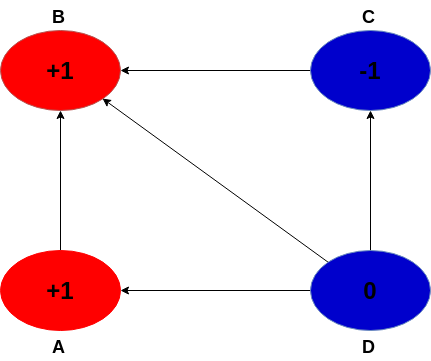
\includegraphics[scale= 0.4]{Passo0.png}
\caption{Passo 0}
\label{Passo0}
\end{minipage}%
\hspace{10mm}%
\begin{minipage}[c]{.40\textwidth}
\centering\setlength{\captionmargin}{0pt}%
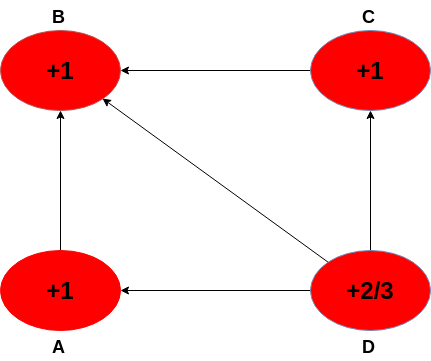
\includegraphics[scale= 0.4]{Passo1.png}
\caption{Passo 1}
\label{Passo1}
\end{minipage}
\hspace{10mm}%
\begin{minipage}[c]{.40\textwidth}
\centering\setlength{\captionmargin}{0pt}%
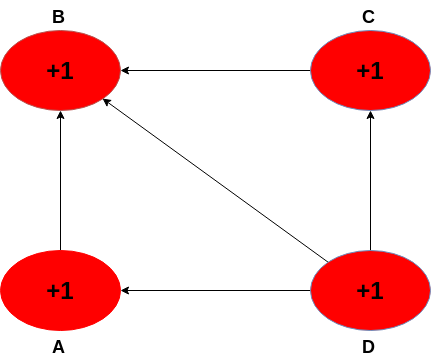
\includegraphics[scale= 0.4]{Passo2.png}
\caption{Passo 2}
\label{Passo2}
\end{minipage}
\hspace{10mm}%
\begin{minipage}[c]{.40\textwidth}
\centering\setlength{\captionmargin}{0pt}%
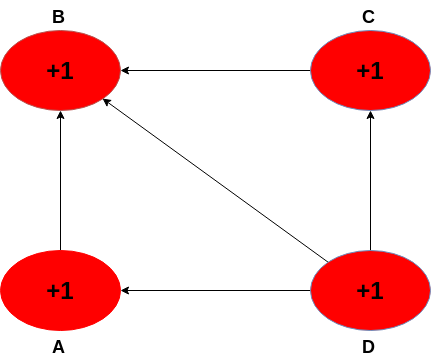
\includegraphics[scale= 0.4]{Passo2.png}
\caption{Passo 3}
\label{Passo3}
\end{minipage}
\caption{Esempio algoritmo basato sul grado}\label{fig:minipage2}
\end{figure}

Dal punto di vista implementativo l'algoritmo trattato è stato implementato mediante le funzionalità contenute all'interno della libreria \textit{NetworkX}, la quale garantisce ottime prestazione nel caricamento dei dati relativa alla matrice di adiacenza, senza far saturare la memoria volatile del sistema.
\newpage
\subsection{Polarizzazione basata sulla topologia}
La polarizzazione basata sulla topologia del grafo è un algoritmo definito all'interno di questo paper:\textit{Reducing Controversy by Connecting Opposing Views}.
L'algoritmo in questione sfrutta la topologia del grafo per poter valutare la polarizzazione di ogni singolo nodo a fronte dell'opinione espressa all'interno del tweet pubblicato.
Per prima cosa una volta costruito l'\textit{endorsement graph} un ruolo fondamentale lo svolge la scelta delle due partizioni che compongono il grafo.
Nel paper in questione le partizioni venivano effettuate attraverso una catalogazione degli hashtags, cioè degli elementi testuali che esprimessero in poche parole, o una loro concatenazione, un parere su una determinata notizia.
Per fare un esempio se il topic dell'analisi fosse stata una partita di calcio ed un utente avesse pubblicato un tweet con un hashtag come \textit{\#ForzaBlu}, questo sarebbe stato associato come un parere positivo verso la squadra blu. Però se nel testo ci fosse stata una frase negativa insieme all'hashtag precedente, sarebbe stato un errore perché non più a favore della squadra blu, bensì per il suo avversario. Per risolvere questa problematica la suddivisione è stata effettuata attraverso la \textit{Sentiment Analysis}(vedi sezione n:\ref{Sentiment}, per ulteriori spiegazioni). 
Tornando alla definizione della polarizzazione anche in questo caso tale strumento può assumere un valore contenuto nel seguente range:
\begin{equation}
[-1,1]
\end{equation}
La polarizzazione applicando quanto illustrato in questo paper risulta essere:
\begin{quote}
Il tempo atteso per un random walk per raggiungere un nodo di grado massimo appartenente ad un insieme X ed Y partendo rispettivamente da un nodo \textit{u}. Otteniamo così:
\[
\begin{cases}
    \rho^{X}(u) \in [0,1]       & \quad \\
     \rho^{Y}(u) \in [0,1]   & \quad 
  \end{cases}
\]
Rispettivamente i risultati dei random walk per raggiungere i nodi di grado massimo di X ed Y\footnote{Per X e Y sono da intendere come le due partizioni ottenute attraverso la sentiment analysis.}. 
Infine definiamo la polarizzazione come:
\begin{equation}\label{polar}
P_{u}= \rho^{X}(u)-\rho^{Y}(u) \ \in [-1,1] 
\end{equation}
\end{quote}
In caso di nodi che non hanno uscite, cioè quei nodi che non hanno alcun arco uscente che gli permetta di comunicare con altri, questi assumeranno il comportamento di nodi di \textit{dangling}, cioè quei nodi che non hanno possibilità di comunicazione. Per dar loro un valore della polarizzazione gli verrà assegnato il valore massimo a seconda della partizione a cui sono associati.
Un discorso analogo è valido anche per i nodi di grado massimo, questi al passo iniziale hanno una polarizzazione pari al valore massimo del loro insieme di appartenenza, però se hanno degli archi in uscita, che li metta in contatto con nodi di opinione opposta, allora tale valore verrà aggiornato attraverso l'algoritmo precedentemente illustrato.


All'interno della tesi sono state affrontate diverse problematiche per la realizzazione di questo algoritmo, per prima cosa è stata inserita la \textit{probabilità di retweet} per calcolare la polarizzazione. In questo modo è stata assegnata una forte relazione tra i nodi che retwettano notizie e quelli che le pubblicano. Nel calcolo del random walk il numero di passi dipende dalla probabilità che relaziona i due nodi, rendendo il calcolo più verosimile alla realtà.
Per completezza si definisce \textit{probabilità di retweet}:
\begin{quote}
Si definisce tale il rapporto che intercorre tra il numero dei retweet che l'utente ha effettuato su un nodo\footnote{Per nodo ci si riferisce ad un tweet pubblicato da un utente} con il numero di retweet totali effettuati dall'utente stesso.
\begin{equation}
 P(retweet)_{ij} = \dfrac{\#retweet_{ij}}{\#retweet_{j}} 
\end{equation}
 con i,j= nodi adiacenti appartenenti al grafo.
 \end{quote}

Detto ciò illustriamo un esempio dell'applicazione di questo algoritmo, per completezza consideriamo lo stesso grafo utilizzato in precedenza (vedi fig:\ref{Passo3}):
\begin{figure}[htbp]
    \begin{center}
      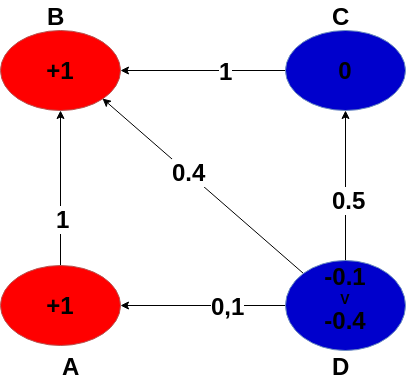
\includegraphics[scale= 0.6]{RWPasso0.png}
		\caption{esempio di polarizzazione basata sulla topologia}
	\label{RandomWalk}
    \end{center}
  \end{figure}

Come possiamo notare i nodi di grado massimo della partizione \textit{Rossa} e \textit{Blu} sono rispettivamente i nodi: B e C, perché quelli aventi \textit{indegree} massima per le rispettive partizioni. Le colorazioni sono il risultato della sentiment analysis.
Analizzando i risultati presentati nell'immagine \ref{RandomWalk}, possiamo notare come la probabilità di retweet giochi un ruolo cruciale nell'analisi in questione. 
Possiamo notare un comportamento particolare nel nodo B il quale assume un polarizzazione pari a zero. Essendo un nodo di grado massimo appartenente alla partizione Blu, ha pubblicato notizie a favore di quel gruppo, però ha anche condiviso notizie a favore del gruppo opposto modificando la sua natura originale. In conclusione applicando la formula \ref{polar}, otteniamo un annullamento della sua polarizzazione
%Infatti possiamo notare come il nodo B abbia una polarizzazione pari a zero, ciò è dovuto dal fatto che essendo un nodo di grado massimo appartenente alla partizione Blu, quindi ha pubblicato una notizia inerente a quel gruppo, avendo retwettato un tweet opposto alla sua visione iniziale indica un cambiamento della sua natura e quindi applicando la formula \ref{polar}, otteniamo un annullamento della sua polarizzazione.
Un altro comportamento particolare è osservabile nel nodo D, questi avrà due possibili valori a seconda del percorso scelto durante il random walk. Se consideriamo il percorso per raggiungere il nodo di grado massimo appartenente alla partizione Blu è facile notare che tale valore è pari a:
\[\rho^{Y}(D)= (D,C) = 0.5
\]
Per quanto riguarda la partizione Rossa il discorso non è semplice infatti:

\[
\begin{cases}
    \rho^{X}(D)= (D,B)= 0,4        & \quad \\
     \rho^{X}(D)= (D,A)\times(A,B) = 0,1 \times1 = 0,1     & \quad 
  \end{cases}
\]

In conclusione la sua polarizzazione può assumere questi due valori:
\[
\begin{cases}
    P_{B}= \rho^{X}(D)-\rho^{Y}(D) = 0,4 - 0,5 = -0.1   & \quad \\
     P_{B}= \rho^{X}(D)-\rho^{Y}(D) = 0,1 - 0,5 = -0.4    & \quad 
  \end{cases}
\]
Per concludere dal punto di vista implementativo essendo molto oneroso dal punto di vista della memoria volatile, l'esecuzione di tutti questi random walk per ogni nodo, sono state ottimizzate le operazioni. Piuttosto che utilizzare la matrice di adiacenza si è utilizzato un metodo definito nella libreria \textit{NetworkX} che restituisce i primi vicini dell'algoritmo. Dovendo mantenere in memoria una lista di nodi visitati durante l'esecuzione, al raggiungimento di un nodo di grado massimo viene effettuata una operazione di \textit{free} che consente al processo di deallocare le risorse occupate da tale lista.

\section{Predizione}
\label{Predizione}
La predizione è una tecnica che consente di analizzare il comportamento di serie di dati nel tempo, permettendo di poter predirne il comportamento nell'istante temporale successivo a quello attualmente in vigore.
Per la realizzazione degli algoritmi che hanno consentito di poter realizzare una tale operazione sono state adottate delle tecniche molto conosciute nell'ambito del \textit{Forecasting}.
Nello sviluppo di questa tesi queste tecniche sono state implementate per consentire una predizione della polarizzazione di ogni nodo nel mese successivo a quello calcolato. Per mantenere i dati e averli sempre a disposizione, questi sono stati salvati all'interno di file \textit{csv} per poter consentire all'utente di poterli analizzare e consultare nel tempo.
\subsection{Double Exponential Smoothing}
Il Double Exponential Smoothing è una tecnica che sfrutta la serie temporale dei dati raccolti, assegnando una crescita esponenziale sui dati nel tempo, tenendo conto anche del trend di crescita o di decrescita nel tempo. In questo modo si cerca di predire il contenuto nel primo instante successivo.
Questa tecnica è uno sviluppo della semplice Exponential Smoothing che faceva la previsione del singolo punto senza tenere conto del trend che veniva a generarsi tra i diversi punti. 
La polarizzazione cambiava in base ai nuovi collegamenti che venivano a generarsi volta per volta nel tempo, per cui avere una cognizione sul trend della serie numerica risulta molto importante.
Per meglio comprendere il funzionamento di questa tecnica, verrà illustrata la \textit{Exponential Smoothing}:
\begin{equation}\label{singleExp}
\widehat{y}_{x}= \alpha y_{x} + (1-\alpha)\widehat{y}_{x-1}
\end{equation}
Che definisce la relazione che intercorre tra l'instante attuale con quello precedente. Possiamo notare la presenza della costante $\alpha$ che viene definita come \textit{fattore di smoothing}. Fondamentalmente viene effettuata una \textit{Moving average} (vedi sezione n:\ref{moving}), utilizzando i fattori: $\alpha$ ed $(1-\alpha)$.
Analizzando la formula si può notare la presenza di una operazione ricorsiva assumendo il comportamento di un esponenziale.
Il fattore di smoothing assegna un peso all'osservazione più recente rispetto all'ultimo valore precedentemente osservato. In conclusione più $\alpha$ è alto e maggiore e più velocemente il metodo dimentica il passato\footnote{Indica un tasso di decadenza della memoria}.
Alla luce di quanto illustrato con la Exponential Smoothing, è intuibile che la presenza di un trend di analisi diventa fondamentale per un'analisi a lungo termine. La polarizzazione è uno strumento a lungo termine che può rivelare il futuro andamento delle opinioni degli utenti nella rete.
Definiamo la Double Exponential Smoothing come:
\[
\begin{cases}
    l_{x}= \alpha y_{x} +(1-\alpha)(l_{x-1}+ b_{x-1}) \ livello        & \quad \\
    b_{x}= \beta (l_{x}-l_{x-1}) +(1-\beta)b_{x-1}  \ trend        & \quad \\
   \widehat{y}(x+1)=  l_{x} + b_{x} \ forecast    & \quad 
  \end{cases}
\]
Il \textit{livello} espresso nella prima equazione del sistema è simile alla equazione \ref{singleExp}, con la differenza che l'osservazione precedente tiene conto anche dell'andamento (trend) dell'istante precedente.
Il \textit{trend} indica la pendenza della funzione, dal punto di vista matematico e geometrico è assimilabile al \textit{coefficiente angolare} di una funzione.
\begin{equation}
m=\dfrac{\Delta_{y}}{\Delta_{x}}
\end{equation}
Dove $\Delta_{y}$ e $\Delta_{x}$ sono rispettivamente le differenze delle ordinate e delle ascisse tra due punti. Però dal punto di vista del Double Exponential Smoothing, possiamo assumere come la differenze tra le ascisse sia pari ad uno essendo una serie temporale, la differenza tra l'istante attuale e quello precedente è un 1. in conclusione avremo che 
\begin{equation}
m=\dfrac{\Delta_{y}}{1}= y_{x}-y_{x-1}
\end{equation}
Per comodità verrà indicata con  $b_{x}$.
Un altro fattore che risulta evidente nel sistema precedentemente illustrato è la presenza di $\beta$, questo viene chiamato \textit{fattore di trend}. Dal punto di vista funzionale si comporta allo stesso modo di $\alpha$ soltanto che si riferisce al trend e non al livello.
Per la realizzazione di tale algoritmo è stata implementata una funzione \textit{Python} che effettuasse tale a calcolo a partire dalla serie di dati calcolati durante le operazioni della polarizzazione.
La serie di dati in questione risultava contenere al massimo 4 elementi, ovvero i mesi scelti per il periodo dell'analisi. Per calcolare il valore successivo laddove mancassero osservazioni precedenti sono state effettuate delle assunzioni:
\begin{itemize}
\item In caso di una singola osservazione, per predire il futuro, non è possibile applicare tale algoritmo per cui si è scelto di restituire come valore il valore della precedente  osservazione.
\item Il numero minimo di osservazioni per effettuare il calcolo con questo algoritmo deve essere pari a 2.
\end{itemize}
In seguito verranno illustrati i risultati ottenuti mediante questo approccio.
\subsection{Linear Regression}
La Regressione Lineare formalizza e risolve il problema di una relazione funzionale tra variabili misurate sulla base di dati campionari estratti da un'ipotetica popolazione infinita. In statistica l'analisi della regressione è associata alla risoluzione del modello lineare.
La regressione consiste nel costruire un modello attraverso cui prevedere i valori di una variabile dipendente o risposta (quantitativa) a partire dai valori di una o più variabili indipendenti o esplicative.
La relazione tra due o più variabili può essere effettuata attraverso modelli matematici, nel nostro caso quello di una \textit{retta}.
La definizione di regressione lineare è:
\begin{equation}
Y_{i}= \beta_{0} + \beta_{1}X_{i} + e_{i}
\end{equation}
\begin{itemize}
\item \textit{i} indica le diverse osservazioni, $i= 1,....,n$, con \textit{n} pari al numero di osservazioni
\item $Y_{i}$ è la variabile dipendente.
\item $X_{i}$ è la variabile indipendente.
\item $\beta_{0} + \beta_{1}X$ è la retta di regressione. 
\item $\beta_{0}$ è l'intercetta, corrisponde al valore medio di \textit{Y} quando \textit{X} è pari a zero.
\item $\beta_{1}$ è il coefficiente angolare, indica come varia \textit{Y} in corrispondenza di una variazione unitaria di \textit{X}.
\item $e_{i}$ è l'errore statistico.

\end{itemize}
Applicando questa formula viene generata una retta che sia più vicina possibile ai punti analizzati. Nel caso della predizione partendo dalla retta, si calcola il valore nell'istante temporale successivo individuato sulla retta. La medesima operazione è stata effettuata per la serie di dati della polarizzazione.
L'implementazione di questa tecnica è stata effettuata mediante la libreria \textit{Python} \textit{numpy}, la quale consentiva attraverso una lista numerica di calcolare la regressione lineare.
Una volta calcolata la retta e quindi la relativa \textit{quota} e \textit{coefficiente angolare}, si è applicata la classica formula geometrica:
\begin{equation}
y=mx+q
\end{equation}
sostituendo il valore di \textit{x} con l'istante temporale che si voleva calcolare, ottenendo la predizione desiderata.
\subsection{Moving Average}
\label{moving}
La moving average  è una tecnica che estende la media aritmetica dei risultati, andando a mediare i risultati all'interno di una finestra mobile.
Concettualmente vengono prelevati i risultati più recenti all'interno della serie temporale, successivamente questi verranno mediati. Il risultato sarà il valore della predizione dell'istante temporale richiesto.
% Vengono prelevati gli ultimi risultati ottenuti mediati ed infine viene definito come valore futuro questo risultato.
Viene anche definita \textit{finestra mobile}, proprio perché calcola la media dei valori all'interno di una finestra limitata rispetto alla serie di dati contenuti.
La definizione matematica è la seguente:
Data una serie storica $y_{t}$, con $\textit{t}= 1,...,T$, contenente i valori osservati di una variabile \textit{Y}  dal tempo 1 al tempo \textit{T}, siano:
\begin{itemize}
\item $m_{1}$ il numero dei periodi precedenti a \textit{t};
\item $m_{2}$ il numero dei periodi successivi a \textit{t};
\item $\theta_{i}$ il peso da attribuire all' \textit{i-esimo} valore osservato;
\end{itemize}
\begin{equation}
Media_{t}= \dfrac{1}{k} \sum_{i=-m_{1}}^{m_{2}}\theta_{i}y_{t+i}
\end{equation}
In conclusione attraverso questa tecnica di forecasting è possibile fare una predizione del valore successivo, attraverso una media tra i valori antecedenti all'evento richiesto. In questo modo viene definita una forte correlazione tra i valori vicini. La moving average è molto utile nel caso si abbiano pochi dati a disposizione.
Dal punto di vista implementativo, utilizzando i dati ottenuto attraverso la polarizzazione, è stato necessario fare delle assunzione:
\begin{itemize}
\item Non è possibile utilizzare questa tecnica con serie numeriche aventi un solo elemento, infatti per sopperire a tale problematica si suppone che la previsione coincida con l'ultimo valore acquisito.
\item La lunghezza massima della finestra temporale, è stata impostata pari a 2 in questo modo si cerca di tener conto del trend ottenuto.
\end{itemize}
In conclusione l'implementazione di tale funzionalità è stata implementata attraverso il \textit{Python}.
